\section{Development \& Results}
\begin{frame}{Development \& Results - Current Progress}
Development is divided into:
\begin{itemize}
    \item EEG MI Classifier
    \item Dataset Augmentation Technique
    \item Virtual Environment
    \item Project Testing Pipeline
\end{itemize}
\end{frame}

\begin{frame}{EEG MI Classifier - Baseline Methods}
    \begin{minipage}[c]{.65\textwidth}
        \begin{itemize}
            \item \textbf{CSP + LDA}: Common Spatial Patterns + Linear Discriminant Analysis
            \item \textbf{TGSP + SVM}: Tangent Space Projection + Support Vector Machine
            \item \textbf{MDM}: Minimum Distance Mean
            \item \textbf{EEGNetV4}: Convolutional Neural Network for Motor Imagery Classification
        \end{itemize}        
    \end{minipage}
    \begin{minipage}[c]{.33\textwidth}
        \begin{figure}[htpb!]
            \centering
            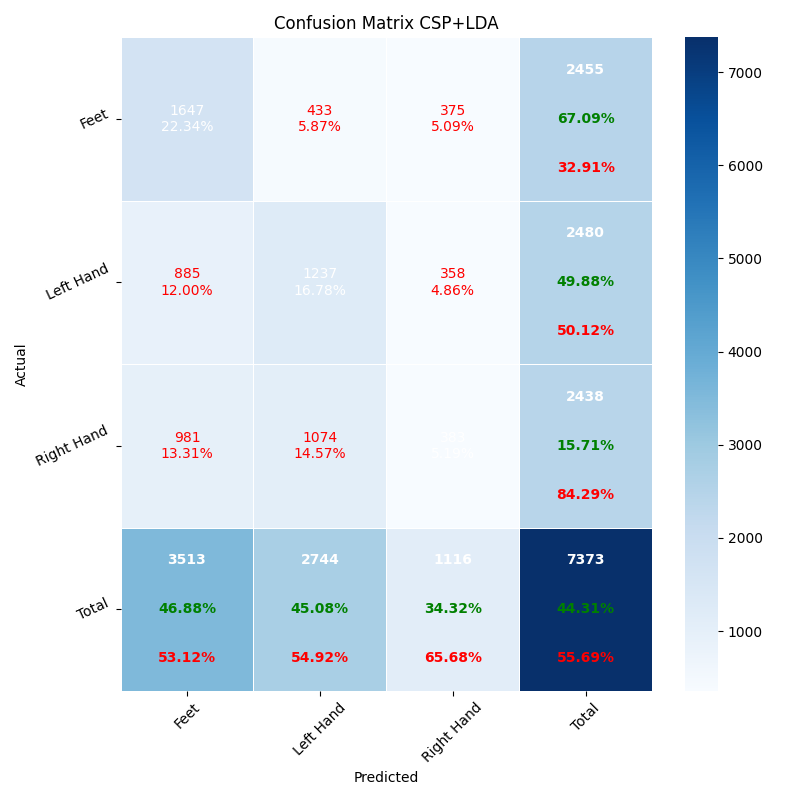
\includegraphics[width=0.45\textwidth]{figures/classification/confusion_matrix_csp_lda}
            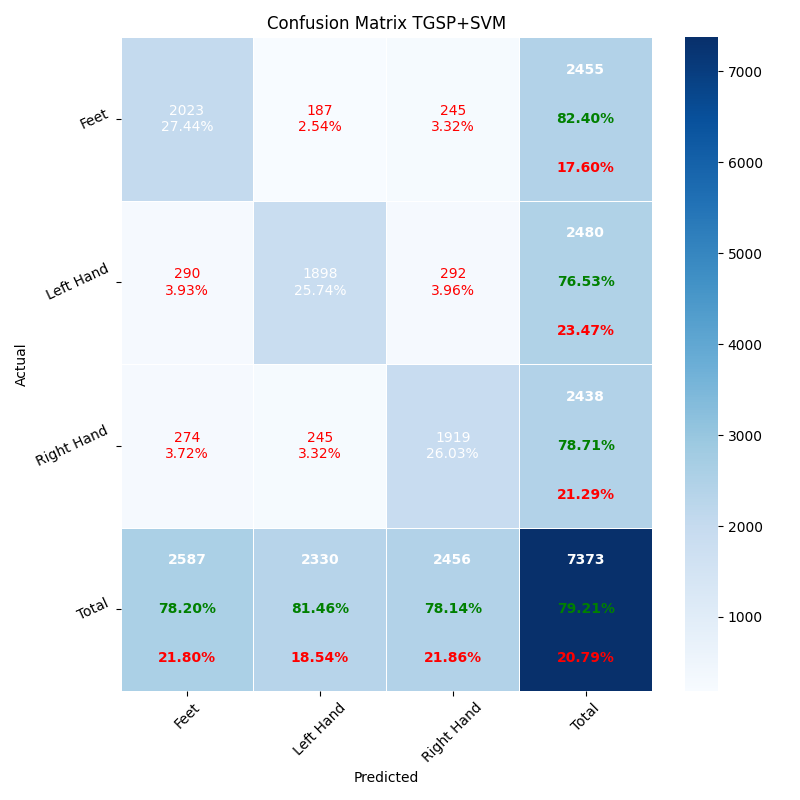
\includegraphics[width=0.45\textwidth]{figures/classification/confusion_matrix_tgsp_svm}
            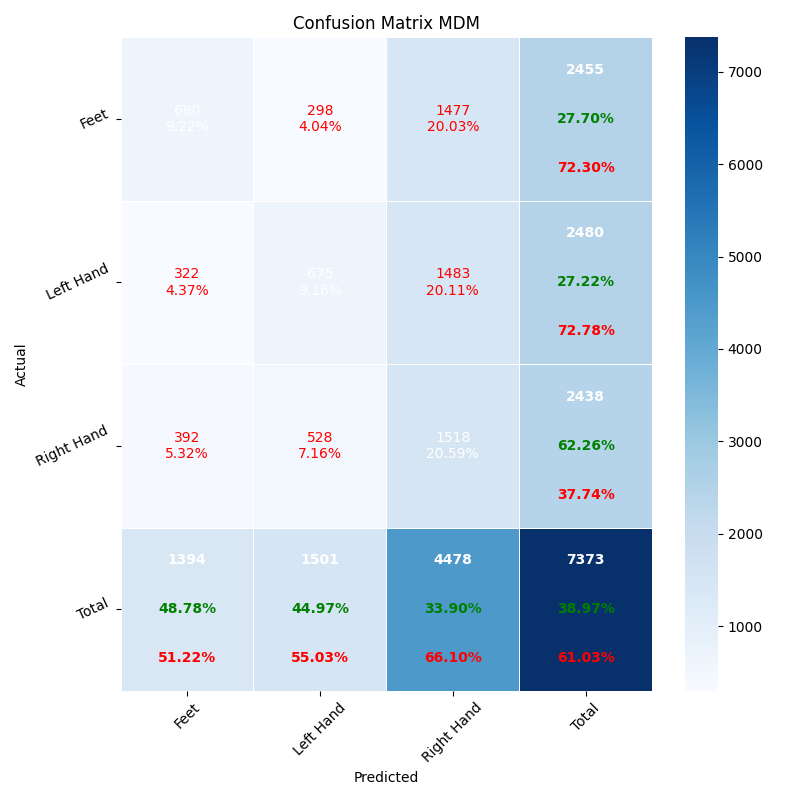
\includegraphics[width=0.45\textwidth]{figures/classification/confusion_matrix_mdm}\\
            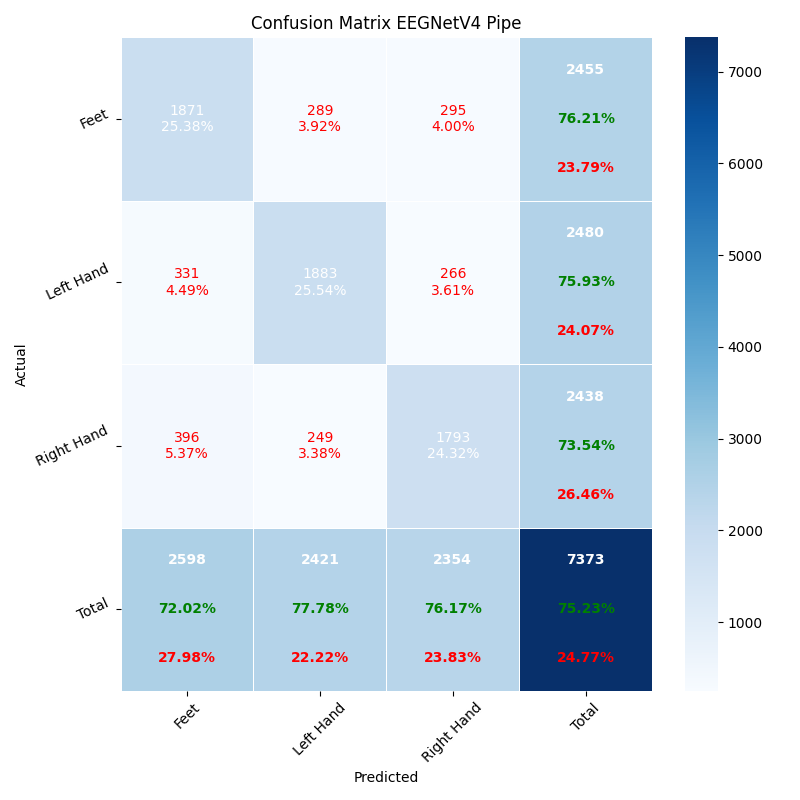
\includegraphics[width=0.45\textwidth]{figures/classification/confusion_matrix_eegnetv4_pipe}
            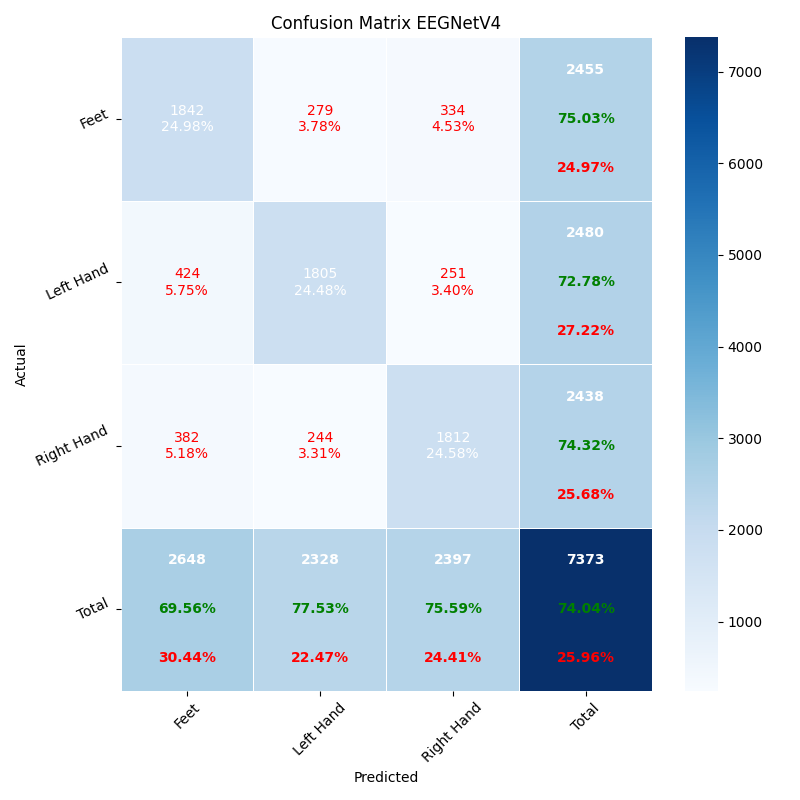
\includegraphics[width=0.45\textwidth]{figures/classification/confusion_matrix_eegnetv4}
        \end{figure}
    \end{minipage}
\end{frame}

\begin{frame}{EEG MI Classifier - Proposed Method}
    \begin{minipage}[c]{.65\textwidth}
        From ``\textbf{Deep temporal networks for EEG-based motor imagery recognition.}'' by \textit{Sharma N. et al.} (2023) I used and adapted: 
        \begin{itemize}
            \item LSTM-based Approach
            \item Transformer-based Approach
        \end{itemize}
    \end{minipage}
    \begin{minipage}[c]{.33\textwidth}
        \begin{figure}[htpb!]
            \centering
            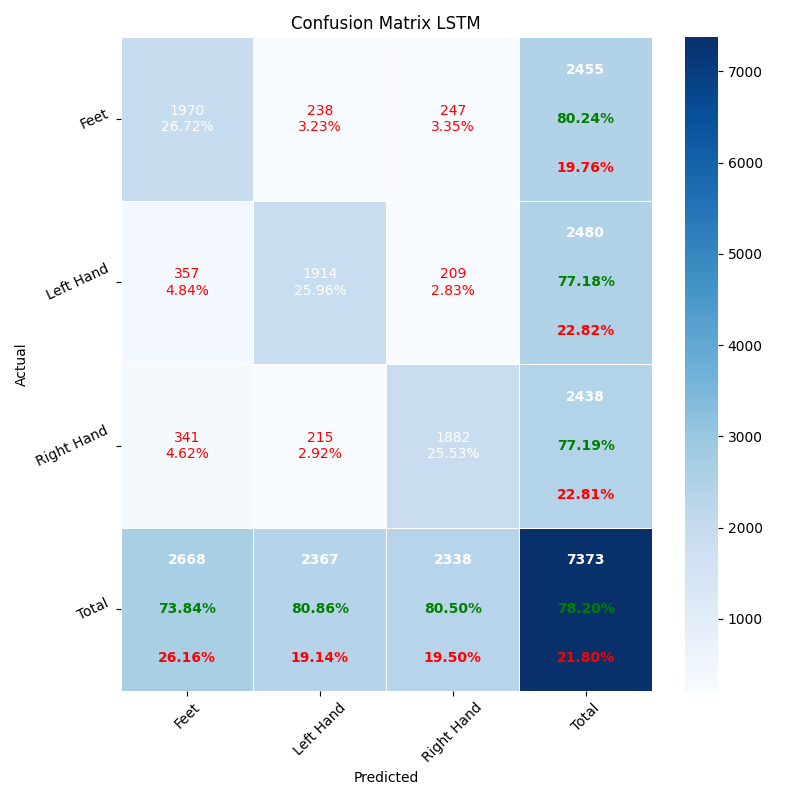
\includegraphics[width=\textwidth]{figures/classification/confusion_matrix_lstm}
            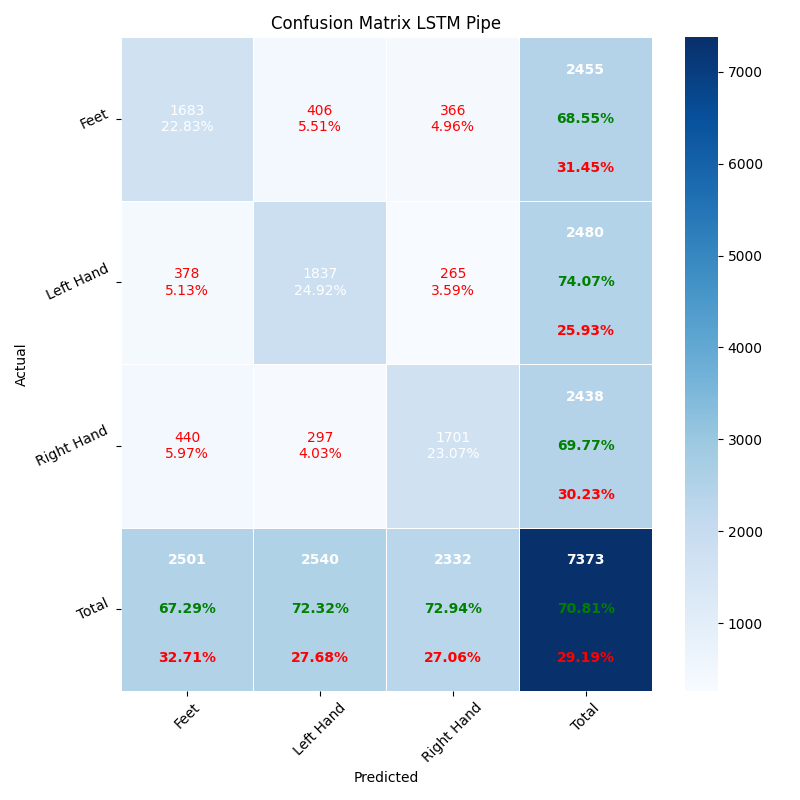
\includegraphics[width=\textwidth]{figures/classification/confusion_matrix_lstm_pipe}
        \end{figure}
    \end{minipage}
\end{frame}

\begin{frame}{Dataset Augmentation - GAN Based}
    \begin{minipage}[c]{.65\textwidth}
        From ``\textbf{EEGFuseNet: Hybrid Unsupervised Deep Feature Characterization and Fusion for High-Dimensional EEG With an \#Application to Emotion Recognition.}'' by \textit{Z. Liang et al.} (2021) I used and trained the network:
        \begin{itemize}
            \item GAN based Approach $\rightarrow{}$ EEGFuseNet
        \end{itemize}
    \end{minipage}
    \begin{minipage}[c]{.33\textwidth}
        \begin{figure}[htpb!]
            \centering
            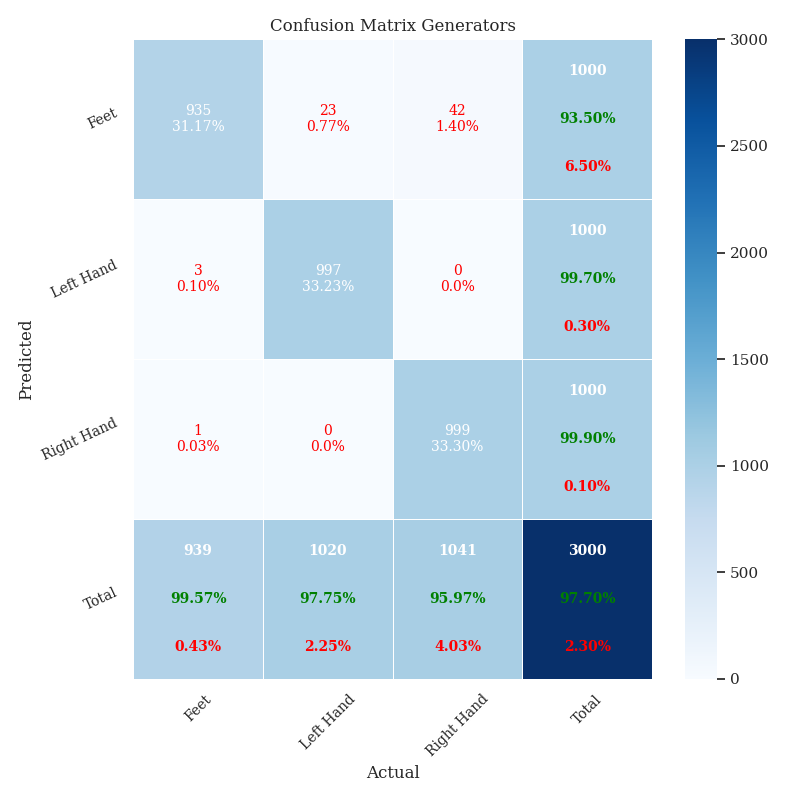
\includegraphics[width=\textwidth]{figures/augmentation/gan/confusion_matrix_generators_generators_using_LSTMNet_0.5943600867678959.pkl}
        \end{figure}
    \end{minipage}
\end{frame}

\begin{frame}{Dataset Augmentation - Stochastic Methods}
    \begin{minipage}[c]{.65\textwidth}            
        From ``\textbf{Data Augmentation for Deep Neural Networks Model in EEG Classification Task: A Review}'' by \textit{C. He et al} (2021) I created a script to generate data using:
        \begin{itemize}
            \item Stochastic Noise Injection Approach\\$\rightarrow{}$ Good Results
            \item Stochastic Generation Approach\\$\rightarrow{}$ Bad Results
        \end{itemize}
    \end{minipage}
    \begin{minipage}[c]{.33\textwidth}
            \centering
            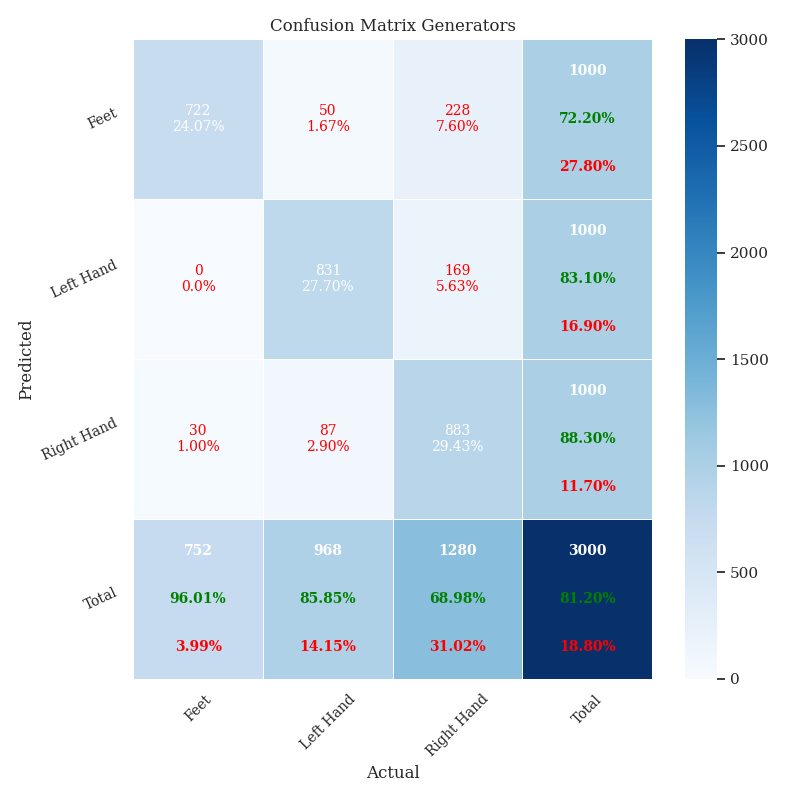
\includegraphics[width=.8\textwidth]{figures/augmentation/stochastic/confusion_matrix_generators_2024_03_30_18_00_20_noise_injector_using_LSTMNet_0.5943600867678959.pkl.png}\\
            {\tiny Noise Injection}\\
            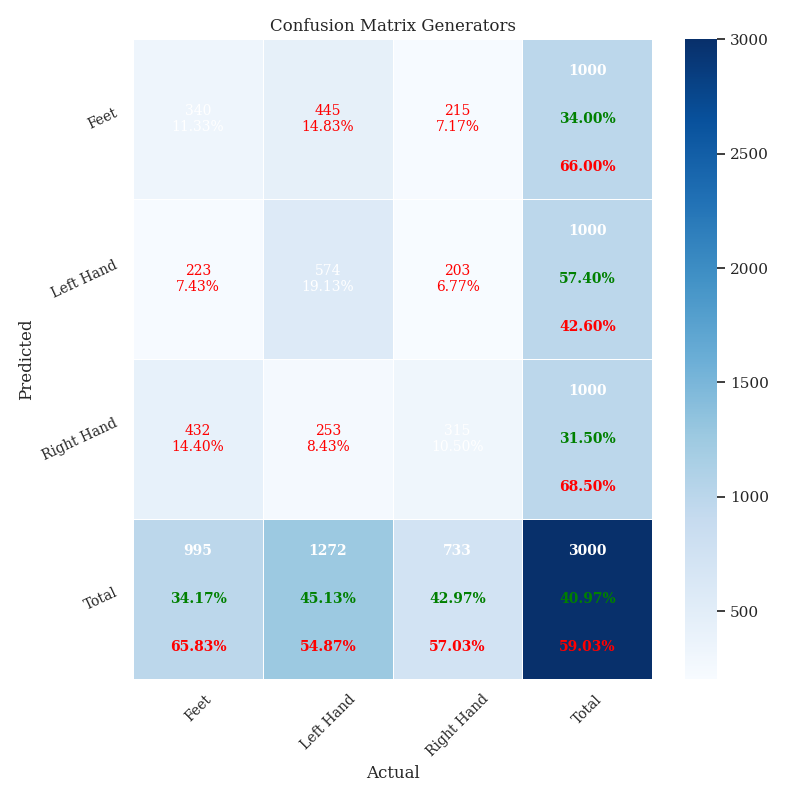
\includegraphics[width=.8\textwidth]{figures/augmentation/stochastic/confusion_matrix_generators_2024_03_30_18_01_19_random_sampler_using_LSTMNet_0.5943600867678959.pkl.png}
            {\tiny Random Sampling}
    \end{minipage}
\end{frame}

\begin{frame}{Project Testing Pipeline}
    \begin{minipage}[c]{.65\textwidth}
        \begin{itemize}
            \item Keyboard Controls (W/Space, A, D)
            \item EEG Signals Generation (Feet, Left Hand, Right Hand)
            \item Signal Classification
            \item Classification Transmission\\(Via WebSocket)
            \item Virtual Character Control
        \end{itemize}
    \end{minipage}
    \begin{minipage}[c]{.33\textwidth}
        \begin{figure}[htpb!]
            \centering
            \href{https://youtu.be/13iwuG1pyk0}{%
            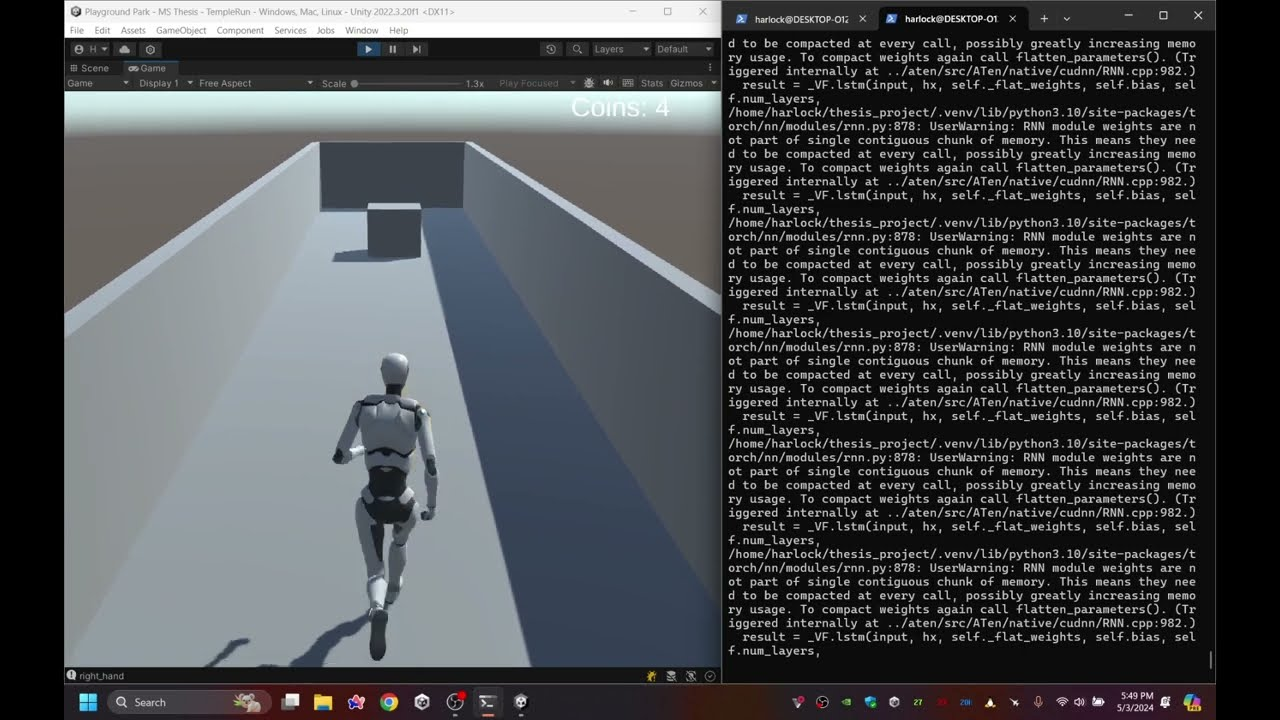
\includegraphics[width=\textwidth]{figures/gameplay/infinite_runner}%
            }
        \end{figure}
        \begin{figure}[htpb!]
            \centering
            \href{https://youtu.be/aBgP87yz1Lw}{%
            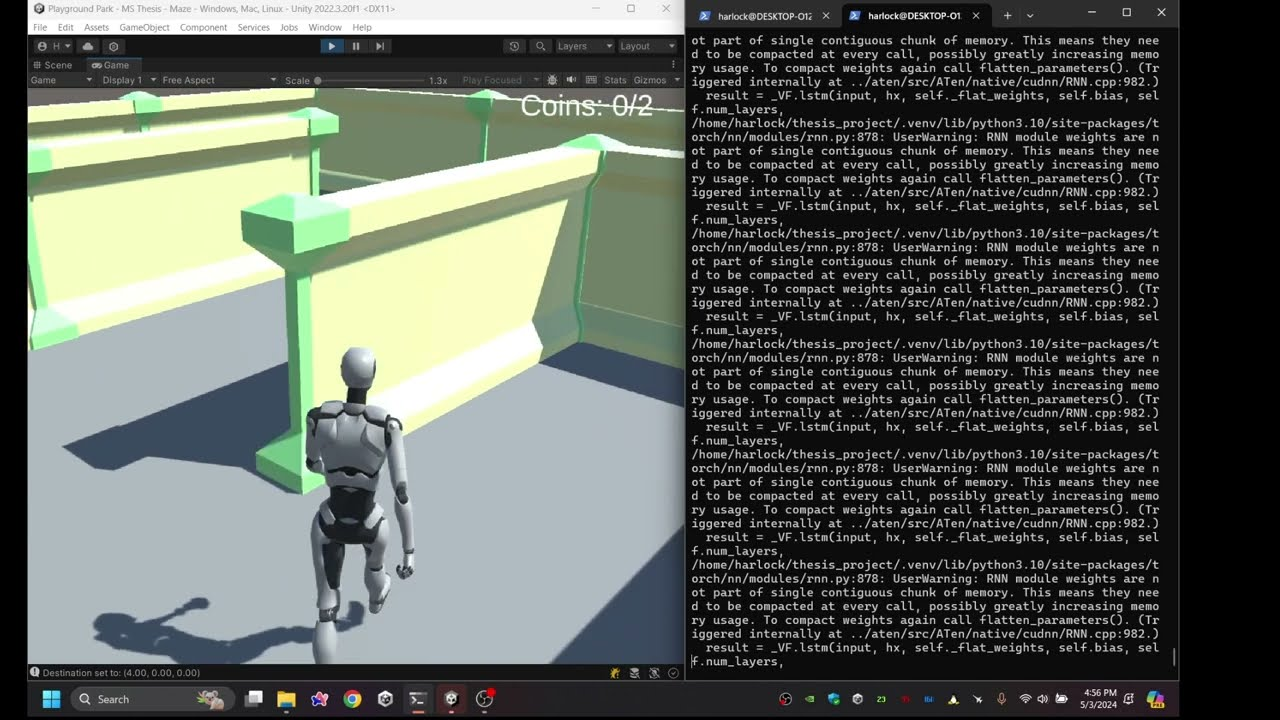
\includegraphics[width=\textwidth]{figures/gameplay/maze}%
            }
        \end{figure}
    \end{minipage}
\end{frame}

\begin{frame}{Pipeline Timeline}
    % using the following time durations create a sequential timeline using tikz
    % from 13 to 80 ms time to process seen image to recognise objects
    % from 100 to 140 ms to generate a motor response
    % 500 ms motor response recording
    % from 1 to 12 ms to classify a signal
    % <1 ms to send the signal to the application

    \begin{tikzpicture}
        % Horizontal line
        \draw[thick] (0,0) -- (7.6625,0);
        \draw[thick, dashed] (7.6625,0) -- (8.15,0);
        \draw[thick, -Triangle] (8.15,0) -- (10,0);
        % \draw[thick, dashed] (9,0) -- (9.5,0);
        % \draw[thick, -Triangle] (9,0) -- (10,0) node[font=\scriptsize,below left=3pt and -8pt]{\textbf{ms}};

        % Start of the timeline
        \draw (0,-0.1) -- (0,0.1) node[font=\scriptsize,below left=3pt and -6pt]{\textbf{0}};
        \node[font=\scriptsize,left=3pt] at (0,0) [anchor=east]{\textbf{Min}};

        % Image Processing Time
        \draw (0.1625, -0.1) -- (0.1625, 0.1) node[font=\scriptsize,below left=3pt and -10pt]{\textbf{\textcolor{olive}{13}}};
        \fill[purple] (0, 0.2) rectangle (0.1625, 0.4);
        
        % \draw (1, -0.1) -- (1, 0.1) node[font=\scriptsize,below left=3pt and -8pt]{\textbf{\textcolor{red}{80}}};
        % \fill[purple] (0,-0.4) rectangle (1,-0.6);
        
        % Motor Response Time
        \draw (1.4125, -0.1) -- (1.4125, 0.1) node[font=\scriptsize,below left=3pt and -10pt]{\textbf{\textcolor{olive}{113}}};
        \fill[blue] (0.1625, 0.4) rectangle (1.4125, 0.6);

        % \draw (2.75, -0.1) -- (2.75, 0.1) node[font=\scriptsize,below left=3pt and -10pt]{\textbf{\textcolor{red}{220}}};
        % \fill[blue] (1,-0.6) rectangle (2.75,-0.8);

        % Motor Response Recording Time
        \draw (7.6625, -0.1) -- (7.6625, 0.1) node[font=\scriptsize,below left=3pt and -8pt]{\textbf{\textcolor{olive}{613}}};
        \fill[red] (1.4125, 0.6) rectangle (7.6625, 0.8);

        % \draw (9, -0.1) -- (9, 0.1) node[font=\scriptsize,below left=3pt and -10pt]{\textbf{\textcolor{red}{720}}};
        % \fill[red] (2.75,-0.8) rectangle (9,-1);

        % Signal Classification Time
        \draw (8.15, -0.1) -- (8.15, 0.1) node[font=\scriptsize,below left=3pt and -10pt]{\textbf{\textcolor{olive}{614}}};
        \fill[amethyst] (7.6625, 0.8) rectangle (8.15, 1);

        % \draw (9.5, -0.1) -- (9.5, 0.1) node[font=\scriptsize,below left=3pt and -10pt]{\textbf{\textcolor{red}{732}}};
        % \fill[amethyst] (9,-1) rectangle (9.5,-1.2);

        % diff curly brace
        % \draw [decorate,decoration={brace,amplitude=5pt}] (8.15, 1) -- (9.5,1) node [anchor=south,midway,above=4pt] {\footnotesize Signal Received by Application};
    \end{tikzpicture}
    \begin{tikzpicture}
            % Horizontal line
            \draw[thick] (0,0) -- (9,0);
            % \draw[thick, dashed] (7.6625,0) -- (8.15,0);
            % \draw[thick] (8.15,0) -- (9,0);
            \draw[thick, dashed] (9,0) -- (9.5,0);
            \draw[thick, -Triangle] (9.5,0) -- (10,0) node[font=\scriptsize,below left=3pt and -8pt]{\textbf{ms}};
    
            % Start of the timeline
            \draw (0,-0.1) -- (0,0.1) node[font=\scriptsize,below left=3pt and -6pt]{\textbf{0}};
            \node[font=\scriptsize,left=3pt] at (0,0) [anchor=east]{\textbf{Max}};
    
            % Image Processing Time
            % \draw (0.1625, -0.1) -- (0.1625, 0.1) node[font=\scriptsize,below left=3pt and -10pt]{\textbf{\textcolor{olive}{13}}};
            % \fill[purple] (0, 0.2) rectangle (0.1625, 0.4);
            
            \draw (1, -0.1) -- (1, 0.1) node[font=\scriptsize,below left=3pt and -8pt]{\textbf{\textcolor{red}{80}}};
            \fill[purple] (0,0.2) rectangle (1,0.4);
            
            % Motor Response Time
            % \draw (1.4125, -0.1) -- (1.4125, 0.1) node[font=\scriptsize,below left=3pt and -10pt]{\textbf{\textcolor{olive}{113}}};
            % \fill[blue] (0.1625, 0.4) rectangle (1.4125, 0.6);
    
            \draw (2.75, -0.1) -- (2.75, 0.1) node[font=\scriptsize,below left=3pt and -10pt]{\textbf{\textcolor{red}{220}}};
            \fill[blue] (1,0.4) rectangle (2.75,0.6);
    
            % Motor Response Recording Time
            % \draw (7.6625, -0.1) -- (7.6625, 0.1) node[font=\scriptsize,below left=3pt and -8pt]{\textbf{\textcolor{olive}{613}}};
            % \fill[red] (1.4125, 0.6) rectangle (7.6625, 0.8);
    
            \draw (9, -0.1) -- (9, 0.1) node[font=\scriptsize,below left=3pt and -10pt]{\textbf{\textcolor{red}{720}}};
            \fill[red] (2.75,0.6) rectangle (9,0.8);
    
            % Signal Classification Time
            % \draw (8.15, -0.1) -- (8.15, 0.1) node[font=\scriptsize,below left=3pt and -10pt]{\textbf{\textcolor{olive}{614}}};
            % \fill[amethyst] (7.6625, 0.8) rectangle (8.15, 1);
    
            \draw (9.5, -0.1) -- (9.5, 0.1) node[font=\scriptsize,below left=3pt and -10pt]{\textbf{\textcolor{red}{732}}};
            \fill[amethyst] (9,0.8) rectangle (9.5,1);
    
            % diff curly brace
            % \draw [decorate,decoration={brace,amplitude=5pt}] (8.15, 1) -- (9.5,1) node [anchor=south,midway,above=4pt] {\footnotesize Signal Received by Application};    
    \end{tikzpicture}
    \begin{itemize}
        \item \textcolor{purple}{Brain Processing Image Time:} 13-80 ms
        \item \textcolor{blue}{Brain Motor Response Activation Time:} 100-140 ms
        \item \textcolor{red}{BCI Motor Response Recording Time:} 500 ms
        \item \textcolor{amethyst}{Signal Classification Time:} 1-12 ms
        \item Classification Sent to Application: $\approx$1 ms (localhost)
    \end{itemize}
\end{frame}
